%!TEX root = synthese.tex
\newpage
\section{Design Pattern - Command}

\subsection{Objectifs}

Les objectifs de l'incrément 4 sont les suivants :\\
\begin{itemize}
\item Réutiliser les traitements interprétés par le terminal;
\item Exprimer de manière unique le traitement des commandes ls et cat.\\
\end{itemize}

Pour cet incrément, nous utiliserons le pattern Command. En effet ce pattern est bien adapté à notre problème car il permet d’isoler une requête. Ces requêtes peuvent provenir de plusieurs émetteurs (dans notre cas \emph{TerminalOS} et \emph{ExplorerOS}). Ces émetteurs doivent produire la même requête. Enfin ces requêtes doivent pouvoir être annulées. 

\subsection{Implémentation}

Pour implémenter le pattern Command, l’UML de notre application se présentera sous cette forme :

\clearpage

\begin{figure}[!h]
\centering
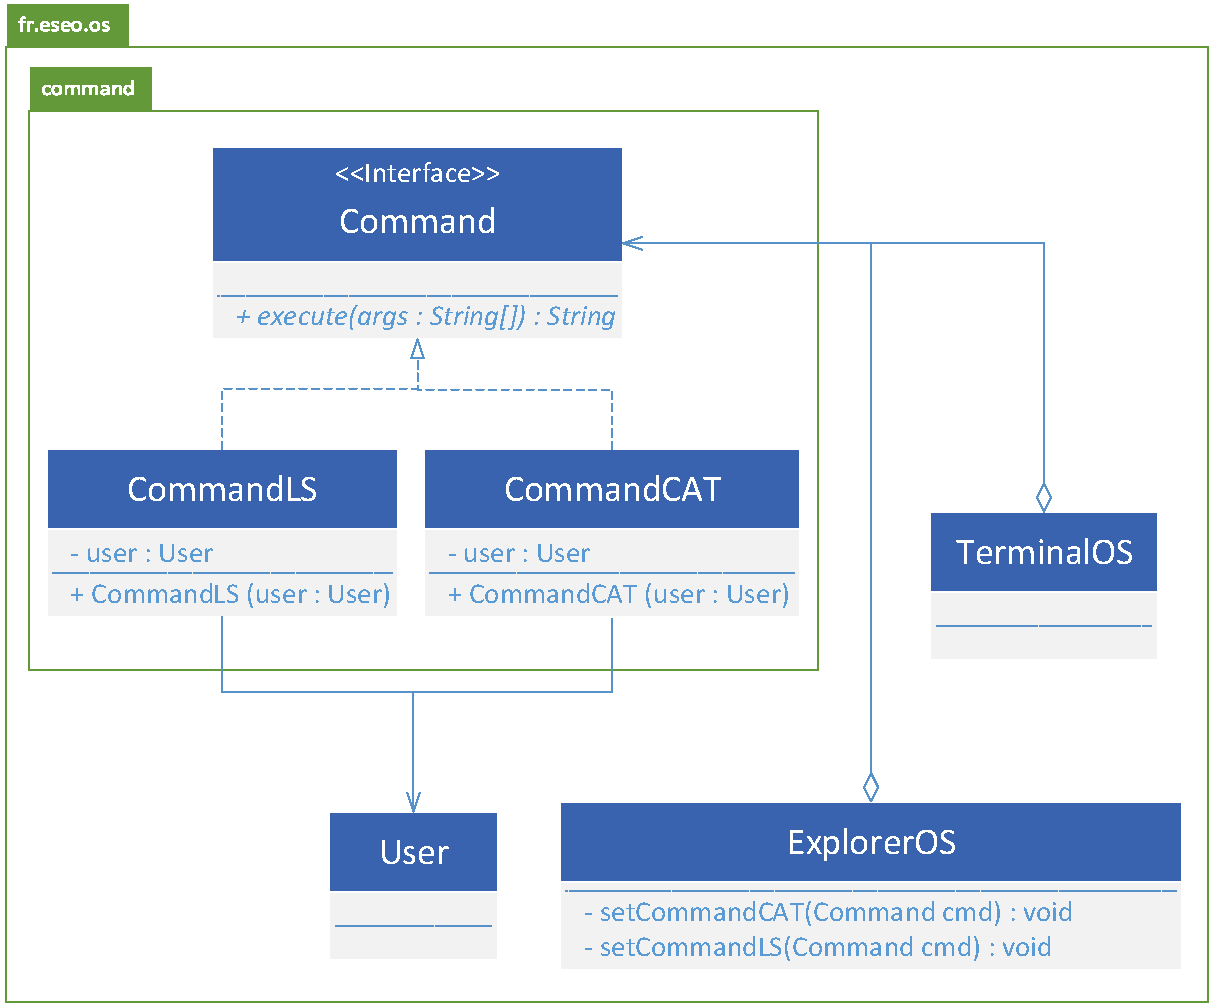
\includegraphics[width=\textwidth]{../uml/uml-command}
\end{figure}

\emph{CommandCAT} et \emph{CommandLS} implémentent l'interface \emph{Commande}. Chaque classe commande implémente la méthode \emph{execute()} de l'interface. Ces méthodes ne font qu'appeler les méthodes \emph{executeCommande()} implémentées dans la classe \emph{User} (le récepteur). Enfin, les classes \emph{TerminalOS} et \emph{ExplorerOS} sont des invocatrices car elles déclenchent les commandes via les classes de type \emph{Command}.\\

Dans un premier temps, nous créons une nouvelle interface emph{Commande} comme suit :

\begin{lstlisting}
package fr.eseo.os.command;
public interface Command {
    String execute(String... args);
}
\end{lstlisting}

Cette interface possède une unique méthode \emph{execute()} car la commande ne réalise pas le traitement, elle est juste porteuse de la requête.  Nos commandes ls et cat seront donc encapsulées dans un objet \emph{Command} et l’interface \emph{Command} sera implémentée par deux classes : \emph{CommandCAT} et \emph{CommandLS}.\\

On définit ensuite deux objets de type \emph{Command} dans \emph{ExplorerOS} et \emph{TerminalOS}.

\begin{lstlisting}
private Command commandCAT;
private Command commandLS;
\end{lstlisting}

On a créé une classe \emph{CommandEnum} afin de lister l'ensemble des commandes.

\begin{lstlisting}
public enum CommandEnum {

    LS ("ls"),
    CAT ("cat"),
    MKDIR ("mkdir"),
    RM ("rm"),
    TOUCH ("touch"),
    LN ("ln"),
    NOT_FOUND ("commande introuvable");

    private String command;

    private CommandEnum(String command){
        this.command = command;
    }

    public String getCommand(){
        return command;
    }

    public static CommandEnum getEnum(String command){
        if (command != null){
            for (CommandEnum value : values()) {
                if (value.getCommand().equals(command)){
                    return value;
                }
            }
        }
        return  NOT_FOUND;
    }
}
\end{lstlisting}

Dans \emph{ExplorerOS}, on modifie la méthode \emph{runCommand()}.

\begin{lstlisting}
@Override
protected String runCommand(String... args) {
	String result = NOT_FOUND.getCommand();
	// followed by the parameters of the command
	if (args.length > 0) {
		switch (CommandEnum.getEnum(args[0])) {
			case LS:
				if (commandLS != null) {
					result = commandLS.execute(args);
				}
				break;
			case CAT:
				if (commandCAT != null) {
					result = commandCAT.execute(args);
				}
				break;
	}
	updateContents();
	return result;
}
\end{lstlisting}

Cette dernière est appelée dans \emph{TerminalOS} :

\begin{lstlisting}
@Override
public String handleCommand(String command){
	String[] args = command.split(" ");
	String result = ((ExplorerOS)this.explorer)
						.runCommand(args);
	this.user.addHistory(command + '\n' + result + 
			'\n' + user.getLogin() + PROMPT, this);
	return result;
}
\end{lstlisting}

Cette méthode fait appel à la méthode \emph{execute} depuis la classe \emph{CommandLS} ou celle de \emph{CommandCAT}.

\begin{lstlisting}
public class CommandLS implements Command {
    private User user;

    public CommandLS(User user) {
        this.user = user;
    }

    @Override
    public String execute(String... args) {
        return user.executeCommandLS(args);
    }
}
\end{lstlisting}

Cette dernière lance la méthode \emph{executeCommandCat/Ls} présente dans \emph{User} définie comme suit :


\begin{lstlisting}
public String executeCommandCAT(String... args) {
    VisitorNode vn = new VisitorCAT();
    return this.executeCommands(vn, args);
}

public String executeCommandLS(String... args) {
    VisitorNode vn = new VisitorLS();
    return this.executeCommands(vn, args);
}

private String executeCommands
				(VisitorNode vn, String... args) {
        String result = "";
        if (args.length > 1) {
            Node node = this.getHomeDir()
            				.findNode(args[1]);
            switch (CommandEnum.getEnum(args[0])) {
                case LS:
                    if (node == null) {
                        result =  args[1]+" not found.";
                    } else {
                        result = node.accept(vn);
                    }
                    break;
                case CAT:
                    if (node == null) {
                        result =  args[1]+" not found.";
                    } else {
                        result = node.accept(vn);
                    }
                    break;
            }
        } else if (args[0].equals(LS.getCommand())) {
            result = this.getHomeDir().accept(vn);
        } else {
            result = args[0] + " missing operand.";
        }
        return result;
    }
\end{lstlisting}

Enfin,  dans \emph{TerminalOS}, on lie les \emph{commandCAT} et \emph{commandLS} dans \emph{ExplorerOS}  grâce à la méthode \emph{setCommandLS/CAT}.

\begin{lstlisting}
commandLS = new ProxyCommandLS(user);
commandCAT = new ProxyCommandCAT(user);
((ExplorerOS)explorer).setCommandLS(commandLS);
((ExplorerOS)explorer).setCommandCAT(commandCAT);
\end{lstlisting}

